\begin{figure}

	\floatbox{figure}[\FBwidth]
	{
		\caption{Meta analysis of correlations with different measures of text comprehension}\label{figure0X}
	}
	{
	\begin{minipage}{0.48\textwidth}
		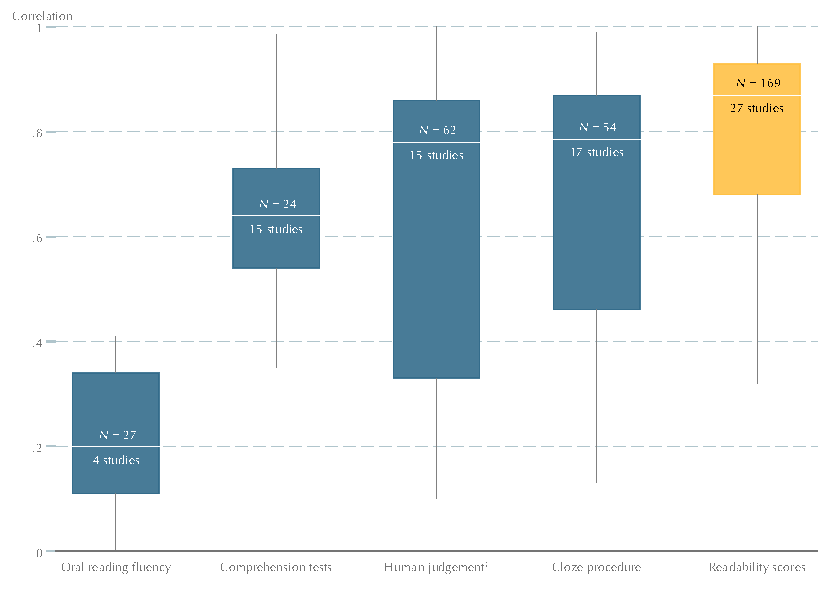
\includegraphics[width=0.95\linewidth]{$HOME/Dropbox/Readability/draft/pdf/figure0X.pdf}
	\end{minipage}
	\begin{minipage}{0.48\textwidth}
		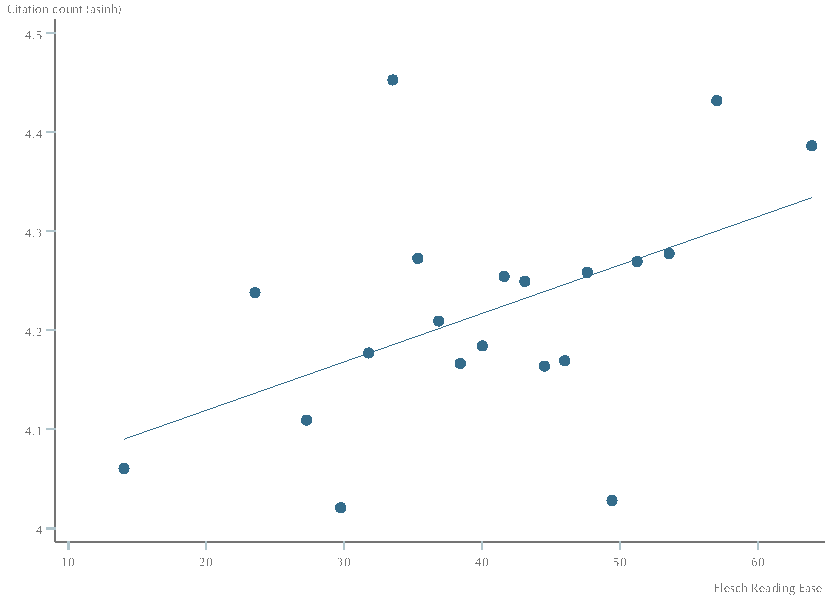
\includegraphics[width=0.95\linewidth]{$HOME/Dropbox/Readability/draft/pdf/asinhCiteCount.pdf}
	\end{minipage}
		\floatfoot{\tiny\textit{Notes}. Graphical display of estimated coefficients of correlation between the five readability scores included in this paper and alternative measures of text comprehension. The figure includes 243 estimates found in 52 separate studies. While I have made every effort to include all relevant studies, the figure is only intended to convey the conclusion that the readability scores used in this analysis are indeed positively correlated with other, arguably more reliable, measures of text difficulty. Please see~\autoref{AppendixMetaAnalysis} for more detailed information of the selection criteria for studies and more detailed information on individual studies.}
	}
\end{figure}